% Тут используется класс, установленный на сервере Papeeria. На случай, если
% текст понадобится редактировать где-то в другом месте, рядом лежит файл matmex-diploma-custom.cls
% который в момент своего создания был идентичен классу, установленному на сервере.
% Для того, чтобы им воспользоваться, замените matmex-diploma на matmex-diploma-custom
% Если вы работаете исключительно в Papeeria то мы настоятельно рекомендуем пользоваться
% классом matmex-diploma, поскольку он будет автоматически обновляться по мере внесения корректив
%

% По умолчанию используется шрифт 14 размера. Если нужен 12-й шрифт, уберите опцию [14pt]
%\documentclass[14pt]{matmex-diploma}
\documentclass[14pt]{matmex-diploma-custom}

\usepackage{listings}
\usepackage{minted}
\usepackage{caption}
\usepackage{subcaption}
\usepackage{amsmath}
\usepackage{csvsimple}

\renewcommand{\lstlistingname}{Листинг}
\renewcommand\listingscaption{Листинг}


\begin{document}
% Год, город, название университета и факультета предопределены,
% но можно и поменять.

\filltitle{ru}{
    chair              = {Кафедра системного программирования},
    title              = {Реализация и оценка эффективности алгоритма обобщенного синтаксического анализа с уменьшенной активностью стека},
    type               = {coursework},
    position           = {студента},
    group              = 344,
    author             = {Ковалев Дмитрий Александрович},
    supervisorPosition = {магистр информационных технологий, ст.\,преп.},
    supervisor         = {Григорьев С.\,В.},
    reviewerPosition   = {},
    reviewer           = {},
    chairHeadPosition  = {},
    chairHead          = {},
%   university         = {Санкт-Петербургский Государственный Университет},
%   faculty            = {Математико-механический факультет},
%   city               = {Санкт-Петербург},
%   year               = {2013}
}

\maketitle
\tableofcontents
\section*{Введение}

Многие существующие сегодня программы во время выполнения формируют из строковых литералов выражения на некотором языке, которые могут переданы для исполнения в соответствующее окружение. Примерами этого могут служить динамическое создание SQL-запросов к базам данных и генерация HTML-страниц.

Одним из недостатков динамической генерации кода является то, что во время компиляции основной программы невозможно провести синтаксический анализ формируемых выражений. Это приводит к отсутствию информации о корректности построенного выражения до момента выполнения программы, что, в свою очередь, существенно увеличивает затраты на разработку и отладку.

Для решения данной проблемы применяют методы статического анализа множества значений динамически формируемого выражения. В рамках исследовательского проекта YaccConstructor \cite{YC} был предложен алгоритм \cite{RelaxedARNGLR} синтаксического анализа регулярной аппроксимации множества значений формируемого выражения. Данный алгоритм позволяет получить компактное представление множества деревьев разбора корректных значений выражения (при этом некорректные значения отбрасываются). 
% * <Семён Григорьев> 14:07:50 31 Aug 2016 UTC+0300:
% RelaxedARNGLR уже опубликован. Надо другую ссылку писать.

Основой для разработанного алгоритма служит RNGLR-алгоритм \cite{rnglr} синтаксического анализа, который позволяет работать с любыми контекстно-свободными грамматиками, в том числе неоднозначными. Для обработки конфликтов, вызванных неоднозначностью грамматики, RNGLR-алгоритм разделяет стек анализатора на две или более ветви, которые в дальнейшей работе также могут быть разделены. Для эффективного представления множества ветвей стека в RNGLR используется специальная структура, называемая структурированным в виде графа стеком (Graph Structured Stack). Несмотря на это, необходимость одновременно работать с многими состояниями стека оказывает существенное влияние на производительность алгоритма.
% * <Семён Григорьев> 14:08:31 31 Aug 2016 UTC+0300:
% Graph Structured Stack -- можно на Томиту сослаться.

В статье Elizabeth Scott и Adrian Johnstone был представлен алгоритм \cite{riglr} синтаксического анализа, позволяющий, как и RNGLR, работать с произвольными КС-грамматиками, при этом значительно сокращая использование стека. Данный алгоритм получил название \textit{Reduction Incorporated Generalized LR (RIGLR)}. Использование RIGLR-алгоритма вместо RNGLR, предположительно, могло быть бы увеличить производительность компоненты, отвечающей за синтаксический анализ динамически формируемых выражений в проекте YaccConstructor.

\section{Постановка задачи}
Целью данной работы является улучшение производительности алгоритма синтаксического анализа динамически формируемого кода.
Для ее достижения были поставлены следующие задачи. 
\begin{itemize}
    \item Изучить RIGLR-алгоритм синтаксического анализа.
    \item Реализовать генератор синтаксических анализаторов, основанный на RIGLR-алгоритме.
    \item Провести сравнение производительности анализаторов, созданных на основе RNGLR и RIGLR.
\end{itemize}

\section{Обзор}
В данном разделе приведен необходимый теоретический материал, дано краткое описание RIGLR-алгоритма, а также описан проект, в рамках которого проводилась его реализация.

\subsection{Контекстно-свободные грамматики и вложенная рекурсия}
\textit{Контекстно-свободная грамматика} $G$ состоит из множества нетерминалов $N$, множества терминалов $T$, такого, что $N \cap T = \emptyset$, стартового нетерминала $S \in N$ и набора правил вида $A ::= \alpha$, где $A \in N$ и $\alpha$ --- строка из терминалов и нетерминалов (возможно пустая).

\textit{Шагом вывода} в грамматике называют выражение вида $\gamma \Rightarrow \delta$, где $\gamma, \delta$ --- строки из терминалов и нетерминалов, и $\delta$ получается из $\gamma$ путем замены нетерминала $A$ на строку $\alpha$, где $A ::= \alpha$ --- правило грамматики. \textit {Вывод} $\delta$ из $\gamma$ --- это последовательность шагов вывода $\gamma \Rightarrow \beta_1 \Rightarrow \beta_2 \Rightarrow ... \Rightarrow \beta_{n - 1} \Rightarrow \delta$.

Говорят, что в грамматике $G$ присутствует \textit{вложенная рекурсия}, если для некоторого нетерминала $A$ и строк $\alpha, \beta \neq \epsilon$, где $\epsilon$ --- обозначение для пустой строки, в этой грамматике существует вывод $A \Rightarrow^* \alpha A \beta$.

\subsection{RIGLR-алгоритм синтаксического анализа}

RIGLR-алгоритм позволяет свести обращения к стеку в процессе анализа к обработке правил, отражающих вложенную рекурсию. Для достижения данного результата алгоритм использует управляющие таблицы, отличные от стандартных LR-таблиц.

Процесс их построения начинается с удаления из исходной грамматики вложенной рекурсии --- если для некоторого нетерминала $A$ существует вывод $A \Rightarrow^* \alpha A \beta$, $\alpha, где \beta \neq \epsilon$, в правой части последнего правила в выводе вхождение $A$ заменяется на особый терминал $A^\perp$. Для примера рассмотрим грамматику правильных скобочных последовательностей (\ref{brackets_gr}), которая после преобразования принимает вид (\ref{brackets_gr_mod}).

Далее, для каждого нетерминала $A$, за исключением стартового, рассматривается грамматика $G_A$ с тем же набором правил, что и в исходной, но со стартовым правилом вида $S_A ::= A$. Для каждой такой грамматики строится \textit{Reduction Incorporated Automaton (RIA)} --- автомат, схожий с LR(0)-автоматом, но включающий в себя особые ребра, соответствующие действиям свертки. 
Наконец, все RIA($G_A$) объединяются в финальный автомат, получивший название \textit{Recursion Call Automaton (RCA)}. Объединение происходит следующим образом: все ребра $(s, t)$ с меткой $A^\perp$ в каком-либо из автоматов удаляются, а вместо них добавляются ребра $(s, startState(RIA(G_A)))$ с меткой $push(t)$. Табличное представление RCA и называют управляющей таблицей RIGLR. 

\begin{listing}[t]
\centering
$\begin{array}{rl}
S \rightarrow ( \ S \ S \ ) \ | \ a \ | \ \epsilon
\end{array}$
\caption{Грамматика $G_0$}
\label{brackets_gr}
\end{listing}

\begin{listing}[t]
\centering
$\begin{array}{rl}
S \rightarrow ( \ S^\perp \ S^\perp \ ) \ | \ a \ | \ \epsilon
\end{array}$
\caption{Грамматика $G_1$}
\label{brackets_gr_mod}
\end{listing}

\begin{figure}[h]
\centering
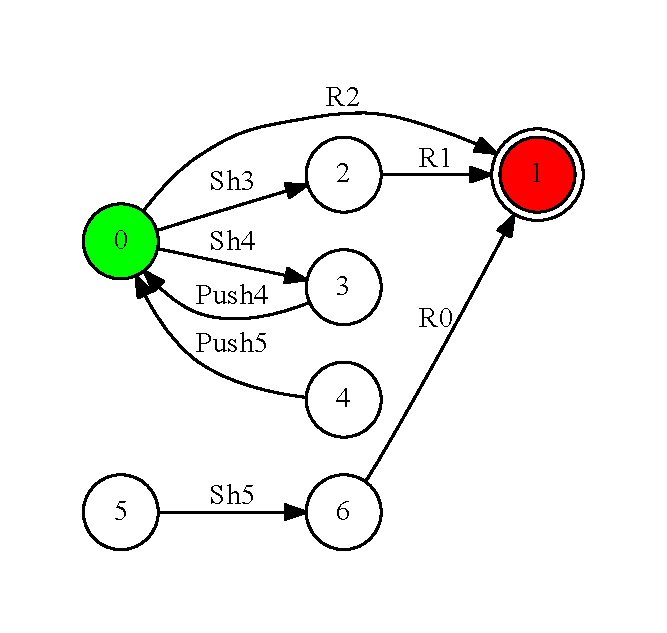
\includegraphics{pictures/RCABrackets.pdf}
\caption{RCA для грамматики $G_1$}
\label{brackets_rca}
\end{figure} 

Стек RIGLR-алгоритма представляется в виде \textit{Recursion Call Graph (RCG)} --- ориентированного графа, вершина которого хранит номер состояния, в которое необходимо совершить возврат после разбора рекурсивного нетерминала. В процессе работы RCG изменяется лишь в том случае, если запись в управляющей таблице для текущих состояния и токена содержит действие $push(l)$ (т.е. в RCA из текущего состояния выходит ребро с меткой $push$), добавляющее в RCG вершину с меткой $l$ и ребро из новой вершины в текущую. Действия переноса и свертки создают узлы в дереве разбора, не модифицируя стек.

Результатом работы RIGLR-анализатора является сжатое представление леса разбора --- \textit{Shared Packed Parse Forest (SPPF)} \cite{sppf}, компактно представляющее все возможные варианты разбора входной цепочки.

\subsection{Проект YaccConstructor}

YaccConstructor (далее YC) \cite{YC} --- исследовательский проект лаборатории языковых инструментов  JetBrains на математико-механическом факультете СПбГУ, направленный на исследования в области лексического и синтаксического анализа, а также статического анализа встроенных языков. Проект включает в себя одноименную модульную платформу для разработки лексических и синтаксических анализаторов, содержащую большое количество компонент: язык описания грамматик YARD, преобразования над грамматиками и др. Основным языком разработки является F$\#$.  

\section{Реализация RIGLR-алгоритма}
% что-то
\subsection{Архитектура}
В рамках данной работы был реализован новый модуль платформы YC, который, в терминах проекта, представляет из себя генератор. На рисунке \ref{YCArch} изображена архитектура платформы, цветом выделен реализованный модуль.

\begin{figure}[h]
\centering
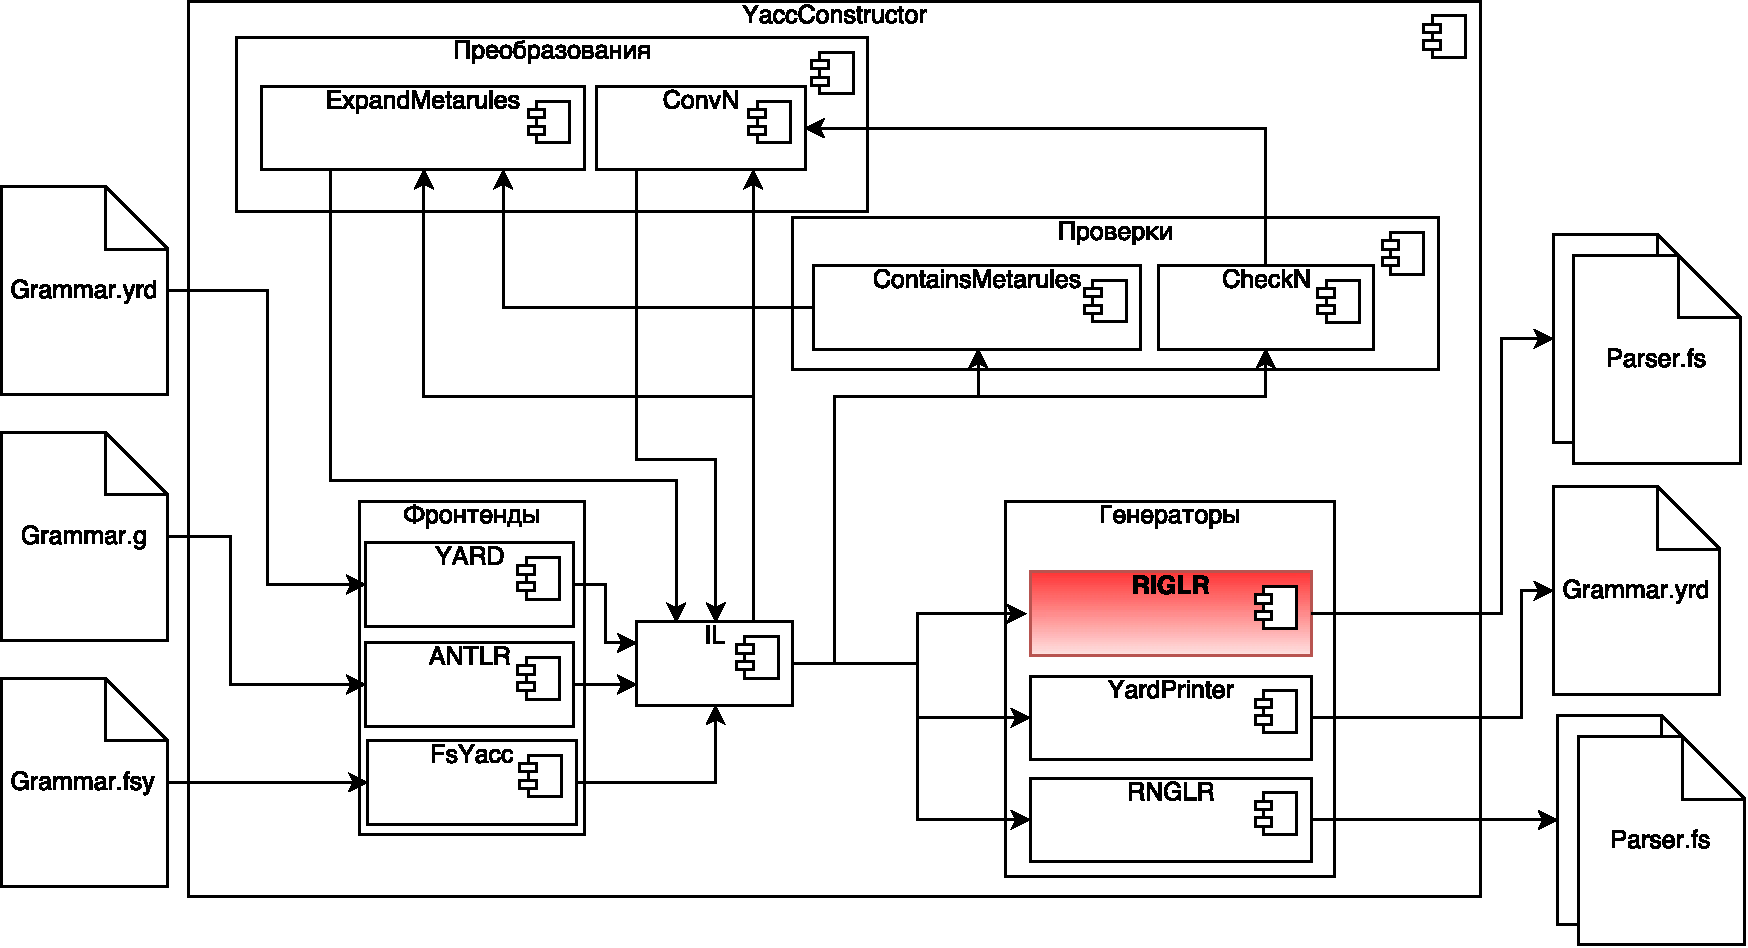
\includegraphics[width=0.9\textwidth]{pictures/YCArch.pdf}
\caption{Архитектура YC}
\label{YCArch}
\end{figure} 

Более подробную структуру модуля можно увидеть на рисунке \ref{RIGLRArch}. Основными компонентами являются генератор, который по входной грамматике создает файл с управляющими таблицами и дополнительной информацией для интерпретатора, и интерпретатор, содержащий основную логику алгоритма и структуры данных, необходимые для его работы.

Пользователь при создании приложения, использующего модуль, добавляет в свой проект сгенерированный файл, ссылку на интерпретатор и файл, содержащий лексический анализатор (полученный с помощью другого модуля YC, который не описывается в данной работе), и вызывает соответствующую функцию для синтаксического анализа.

\begin{figure}[h]
\centering
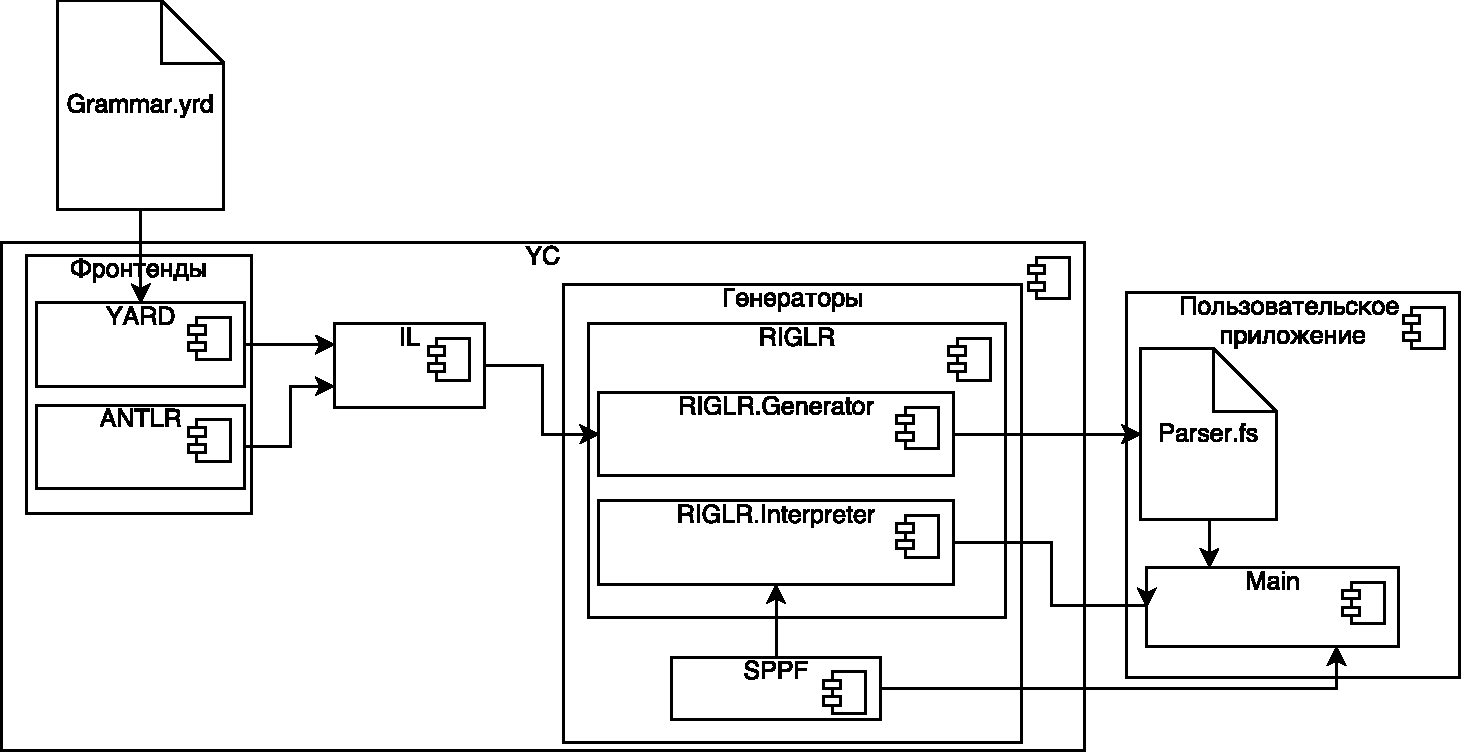
\includegraphics[width=0.9\textwidth]{pictures/RIGLRArch.pdf}
\caption{Архитектура реализованного модуля}
\label{RIGLRArch}
\end{figure} 

\subsection{Модуль генератора}
Модуль генератора содержит в себе реализацию классов автоматов (RIA и RCA), необходимых для построения управляющих таблиц, а также реализацию алгоритма удаления вложенной рекурсии, который основан на алгоритме поиска данного вида рекурсии, описанном в статье \cite{NSE}.

\subsubsection{Реализация RIA и RCA}
Классы, описывающие RIA и RCA, унаследованы от класса FSA<'T> библиотеки QuickGraph \footnote{Проект с открытым исходным кодом. Ссылка --- https://github.com/YaccConstructor/QuickGraph}. Данный класс представляет реализацию конечного автомата с базовым набором функций (например, $\epsilon$-замыканием). RIA и RCA добавляют новые конструкторы, позволяющие инициализировать соответствующий автомат по грамматике, которая была передана как параметр, используя алгоритмы из статьи \cite{riglr}.

\subsubsection{Алгоритм удаления вложенной рекурсии}
Для удаления вложенной рекурсии исходная грамматика представляется в виде \textit{Labelled Production Graph (LPG)} --- помеченного ориентированного графа, вершинами которого являются нетерминалы грамматики, а ребра строятся следующим образом: ребро $A \rightarrow B$ добавляется в граф, если в грамматике существует правило $A \rightarrow \alpha B \beta$. Метка данного ребра определяется так: 

$$ label(A \rightarrow B) = 
\begin{cases}
    L, & \text{если для всех} \ A \rightarrow \alpha B \beta \ \text{выполнено} \ \alpha \neq \epsilon, \beta = \epsilon \\
    R, & \text{если для всех} \ A \rightarrow \alpha B \beta \ \text{выполнено} \ \alpha = \epsilon, \beta \neq \epsilon \\
    B  & \text{в ином случае.}
\end{cases} $$

Путь в графе носит тип $L(R)$, если метки всех ребер в этом пути равны $L(R)$; в ином случае тип пути --- $B$. Нетерминал является самовставленным, если для его вершины существует цикл типа $B$, либо существуют два цикла --- типа $L$ и $R$. Для исключения вложенной рекурсии из грамматики необходимо разомкнуть подобные циклы для всех нетерминалов. 

Реализованный алгоритм разделяет LPG на компоненты сильной связности, затем в каждой компоненте для каждой вершины находит указанные типы циклов при помощи обхода в глубину и размыкает их --- пусть найден цикл для нетерминала $B$ с последним ребром вида $A \rightarrow B$, тогда для всех правил в грамматике вида $A \rightarrow \alpha B \beta$ вхождения $B$ в правой части заменяются на специальный терминал $B^\perp$; ребро удалется из графа.

%пример?
	
\subsubsection{Алгоритм работы генератора}
Общий ход работы генератора выглядит следующим образом:
\begin{itemize}
\item генератор принимает на вход промежуточное представление грамматики, IL, полученное при помощи одного из фронтендов YC из текстового файла соответствующего формата;
\item внутри генератора IL преобразуется в другое представление, называемое FinalGrammar, которое упрощает дальнейшую работу с грамматикой;
\item после получения необходимого представления грамматики, генератор модифицирует ее, удаляя вложенную рекурсию;
\item по грамматике, не содержащей вложенной рекурсии, строится RCA;
\item RCA преобразуется в табличный вид, таблица и дополнительная информация записываются в сгенерированный файл *.fs.
\end{itemize}

\subsection{Модуль интерпретатора}
В модуле интерпретатора находится описание функции \lstinline|buildAst<'T>|, реализующей основную логику RIGLR-анализатора. Функция принимает на вход управляющие таблицы и поток токенов и возвращает лес разбора (SPPF) для данной строки, либо сообщение об ошибке. Модуль переиспользует компоненту с описанием SPPF, реализованную ранее для RNGLR-алгоритма.  

\section{Анализ и сравнение}
Для проведения сравнительного анализа использовалась сильно неоднозначная грамматика, приведенная на листинге \ref{amb}. Данная грамматика инициирует худший случай работы для GLR-алгоритмов.

\begin{listing}[h]
\centering
$\begin{array}{rl}
S \rightarrow  S \ S \ S \ | \ S \ S \ | \ a
\end{array}$
\caption{Грамматика $G_2$}
\label{amb}
\end{listing}

Алгоритмы сравнивались по следующим показателям: размер стека (GSS для RNGLR и RCG для RIGLR; таблица \ref{stack_table}), количество просмотров ребер стека в процессе работы (рис. \ref{edge_visit}), время работы (рис. \ref{time}).

\begin{table}[h]
\centering
\begin{tabular}{|l|l|l|l|l|}
\hline

Токены & RNGLR                  & RIGLR        \\ \hline
10     & 30                         & 20                \\ \hline
20     & 60                         & 40                \\ \hline
30     & 90                         & 60                \\ \hline
40     & 120                        & 80                \\ \hline
50     & 150                        & 100                 \\ \hline
\end{tabular}
\caption{Кол-во вершин в стеке}
\label{stack_table}
\end{table}

\begin{figure}[h]
\centering
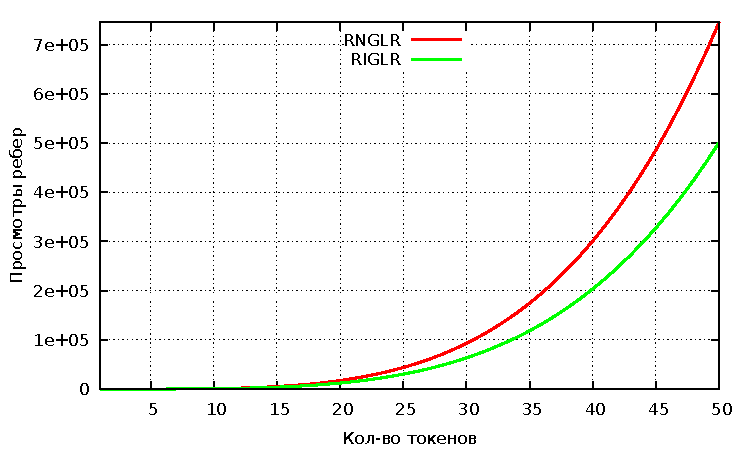
\includegraphics[width=0.8\textwidth]{pictures/edge_visit.pdf}
\caption{Просмотры ребер стека}
\label{edge_visit}
\end{figure} 

В таблице \ref{stack_table} можно увидеть, что количество вершин в стеке RIGLR-алгоритма меньше примерно в $1.5$ раза, что соответствует теоретической оценке из оригинальной статьи. Асимптотическое поведение, выражаемое в количестве просмотров ребер стека, также оказалось лучше для RIGLR, что можно увидеть на рисунке \ref{edge_visit}.

По времени работы RIGLR уступает текущей реализации RNGLR-алгоритма (рисунок \ref{time}). Для увеличения производительности необходима оптимизация структур данных, используемых во время выполнения, и модификация самого алгоритма.

\begin{figure}[h]
\centering
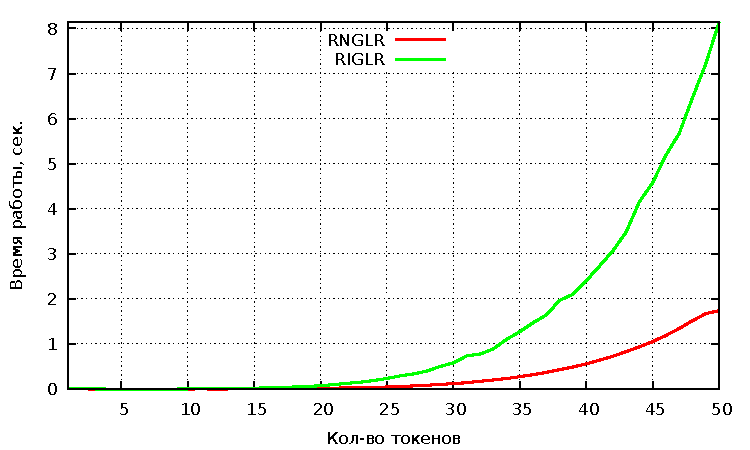
\includegraphics[width=0.8\textwidth]{pictures/time.pdf}
\caption{Время работы алгоритмов}
\label{time}
\end{figure}

\section*{Заключение}
В ходе данной работы получены следующие результаты.
\begin{itemize}
    \item Изучен RIGLR-алгоритм синтаксического анализа.
    \item Реализован генератор синтаксических анализаторов, основанный на RIGLR-алгоритме.
    \item Проведено сравнение производительности анализаторов, созданных на основе RNGLR и RIGLR.
\end{itemize}

В дальнейшем планируется:
\begin{itemize}
\item[---]  увеличить производительность алгоритма, оптимизировав используемые структуры данных;
\item[---] реализовать версию RIGLR-алгоритма, способную производить разбор нелинейного входа, для использования в компоненте анализа динамически формируемого кода.
\end{itemize}

Исходный код данной работы можно найти в репозитории проекта YaccConstructor (\hyperlink{a}{https://github.com/YaccConstructor/YaccConstructor}). Автор работал под учетной записью $Lares77$.


\setmonofont[Mapping=tex-text]{CMU Typewriter Text}
\bibliographystyle{ugost2008ls}
\bibliography{diploma.bib}
\end{document}
